\documentclass[12pt,a4paper]{article}

% --- 日本語設定 -------------------------------------------------------------
\usepackage{luatexja}
\usepackage[haranoaji]{luatexja-preset}


% --- 版面・行間 -------------------------------------------------------------
\usepackage{geometry}
\geometry{top=15mm,bottom=20mm,left=25mm,right=25mm}
\usepackage{setspace}
\onehalfspacing

% --- 数式・図表・表 ---------------------------------------------------------
\usepackage{amsmath,amssymb}
\usepackage{graphicx}
\usepackage{booktabs}

% --- ハイパーリンク ---------------------------------------------------------
\usepackage{xcolor}
\usepackage{svg}
\usepackage{hyperref}
\hypersetup{
    colorlinks=true,       % 枠線ではなく文字を着色
    linkcolor=black,      % 章タイトルなど通常リンクは黒
    urlcolor=blue,        % URL は青
    citecolor=black
}

\usepackage{listings,jvlisting}
\usepackage{enumitem}
\usepackage{multirow}
\usepackage{subcaption}
\usepackage{float}
\usepackage{indentfirst}
\usepackage{pdfpages}


\linespread{1.15}


\renewcommand{\contentsname}{目次}
\renewcommand{\listfigurename}{図目次}
\renewcommand{\listtablename}{表目次}

\renewcommand{\figurename}{図}
\renewcommand{\tablename}{表}
\renewcommand{\refname}{参考文献}



% --- 日本語表記 -------------------------------------------------------------
\makeatletter
\renewcommand{\today}{%
  \number\year 年
  \ifnum\month<10 0\fi\number\month 月
  \ifnum\day<10 0\fi\number\day 日%
}
\makeatother

\title{進捗報告}
\author{下沢\,亮太郎}
\date{\today}


\begin{document}

\maketitle

\section{先週の実施予定内容}

\begin{itemize}
  \item 蒸留元のLLMの選定
  \item 蒸留を検証してみる
\end{itemize}


\section{実施した内容}

\subsection{概要}

引き継いだプロジェクトは，最適化問題100問に対してLLMに\texttt{solve()}コードを生成させ，参照解と照合して採点するものである．
引き継ぎ時点では，DSPy + GEPAによるプロンプト最適化で成績が改善したと報告されていた．
今週は，まず採点系を直し，そのうえで「プロンプト最適化」と「小型モデルへの蒸留」を同じ物差しで比べた．

結果は次の三点である．

\begin{enumerate}
  \item 引き継ぎ時の「GEPAで改善」は採点系の欠陥への適応で，採点系を直すと初期プロンプトと差がなくなった．修正後に再学習したGEPAはQwen3.8でのみ有意に効くが，効果は学習で見た問題種別に限られ，指示文は34KBに膨らむ．
  \item 文脈なしのClaude Fable 5.1が140問中138問を正解した（満点1.5に対し1.494）．この問題集には，プロンプトで伸ばせる余地がそもそも小さい．
  \item 正解コードを教師に4BモデルをLoRA学習すると，学習した28種別の未知instanceではFableと同等（1.487〜1.504）を，1/10の出力量と1/12の時間で達成した．ただし学習していない種別では素のモデルを下回る．
\end{enumerate}


\subsection{採点系の修正}

引き継いだ採点系には，モデル出力と無関係にスコアを歪める欠陥が4つあった（表\ref{tab:scorer}）．
このうちサンドボックスの欠陥が，Phase Eの見かけの優位の主因である．
修正と合わせて，保存済みの生成コードを再実行して採点し直す仕組みを作り，LLMを回さずに全条件を再採点できるようにした．

\begin{table}[H]
  \centering
  \caption{採点系の欠陥と修正}
  \label{tab:scorer}
  \small
  \begin{tabular}{p{0.36\linewidth}p{0.26\linewidth}p{0.28\linewidth}}
    \toprule
    欠陥 & 影響 & 修正 \\
    \midrule
    制約チェッカーが27種別中8種別にしかない & 70問が一律減点（400件中198件がunverified，うち9割は正解） & 20種別のチェッカーを追加．unverified 198 $\rightarrow$ 4 \\
    verifiedフラグが無条件に上書きされる & 不正解に満点 & 上書きを除去 \\
    サンドボックスがscipyのimportとnumpy型を扱えない & 正しいコードが実行エラー & importの解決，numpy値の変換 \\
    参照解と同じ形の解しか読めない & 正しい解をinfeasible判定 & 解析してから検証する形状チェッカー \\
    \bottomrule
  \end{tabular}
\end{table}

評価用の問題集も作り直した．
既存100問のうち28問を雛形に，厳密ソルバー（CP-SAT，線形計画，全列挙）で最適値を計算した新しいinstanceを5問ずつ，計140問生成した．
この140問はGEPAの学習にもdemoにも使っていないホールドアウトで，参照解の正しさが保証されている．
以降の評価はすべてこの140問と修正済み採点系で行い，条件間の差はpaired bootstrapの95\%信頼区間で判定した．

また，Qwen3.8は出力枠32kでは思考が切れて本文が空になる問題が140問中35問で起きたため，比較の既定を出力枠65,536にした．


\subsection{プロンプト最適化（GEPA）の再評価}

指示文の6条件をQwen3.6-27BとQwen3.8-27Bで比べた（表\ref{tab:prompt}，図\ref{fig:score}）．条件は次のとおり．

\begin{itemize}
  \item \textbf{before}：初期指示文
  \item \textbf{Phase E}：引き継いだGEPA学習済み指示文
  \item \textbf{compact}：初期指示文を共通原則だけに圧縮した版
  \item \textbf{modular}：compactに分野別の補足を実行時に足す版
  \item \textbf{再学習GEPA}：compactを初期値に，修正済み採点系で学習し直した版
\end{itemize}

before以外の5条件には，Phase Eの学習でGEPAが選んだfew-shot例2件（demo）を共通で付けた．
before + demoは，demoだけの効果を指示文の効果から切り分けるための対照条件である．

\begin{table}[H]
  \centering
  \caption{生成140問の平均スコア（満点1.5，出力枠65,536）}
  \label{tab:prompt}
  \begin{tabular}{llrr}
    \toprule
    条件 & 指示文 & Qwen3.6 & Qwen3.8 \\
    \midrule
    before & 1.5KB & 1.354 & 1.220 \\
    before + demo & 1.5KB + demo & 1.382 & 1.274 \\
    Phase E（引き継ぎ時） & 17.3KB + demo & 1.396 & 1.306 \\
    compact & 1.8KB + demo & 1.425 & 1.265 \\
    modular & compact + 分野補足 & 1.369 & 1.247 \\
    再学習GEPA & 33.9KB + demo & \textbf{1.440} & \textbf{1.389} \\
    \bottomrule
  \end{tabular}
\end{table}

\begin{figure}[H]
  \centering
  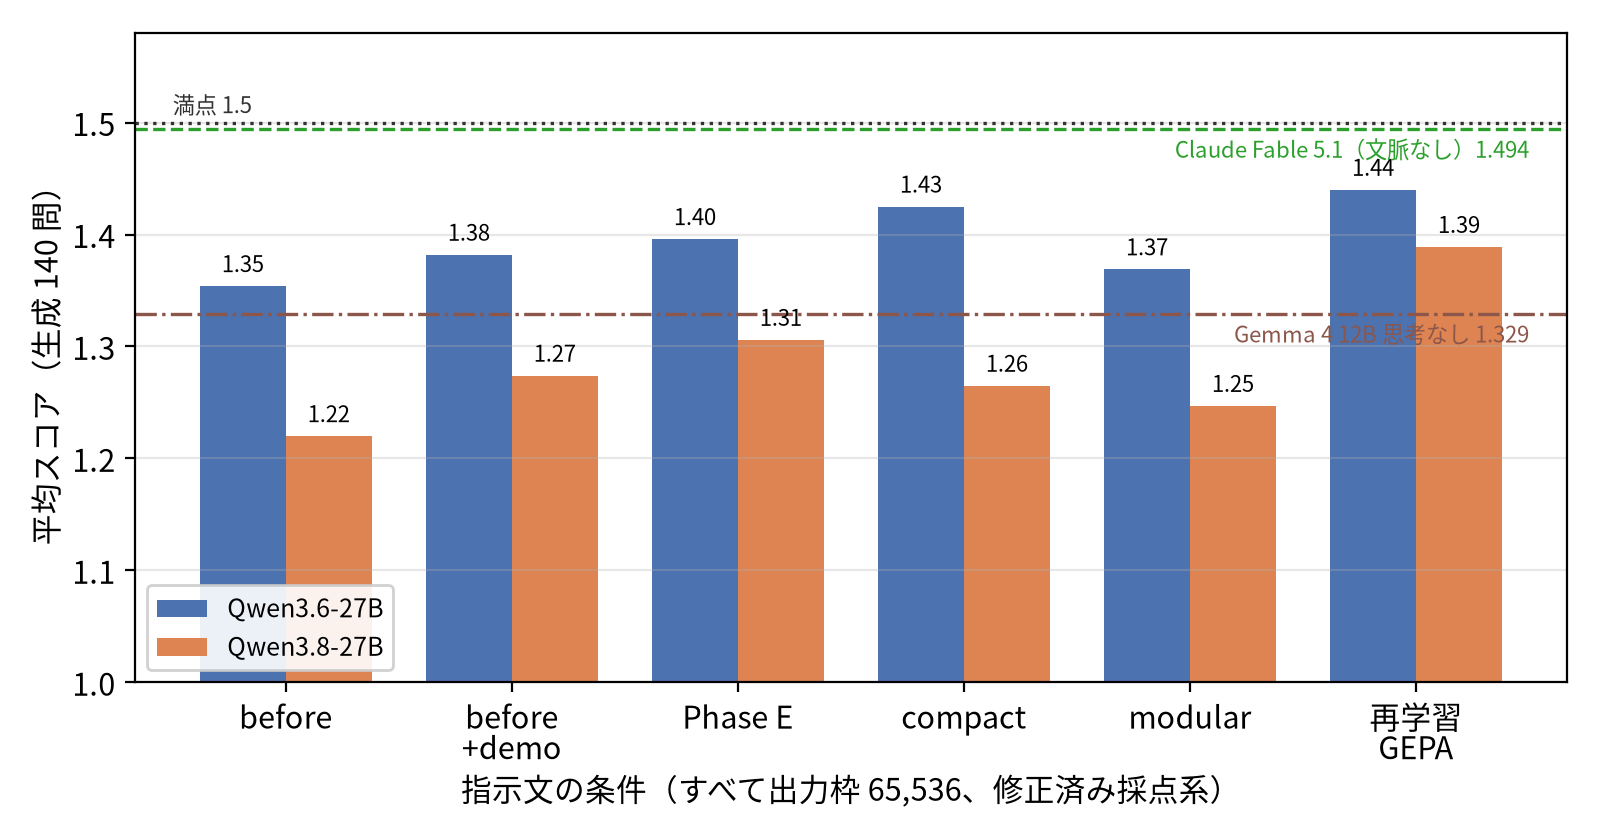
\includegraphics[width=0.95\linewidth]{./assets/score_by_condition.png}
  \caption{生成140問の条件別平均スコア}
  \label{fig:score}
\end{figure}

Phase Eは，before，compact，modularのどれとも有意差がなかった（どちらのモデルでも信頼区間が0を含む）．
引き継ぎ時に報告されていた優位は，採点系の欠陥に適応した結果である．

再学習GEPA（2 GPUで11時間22分）はQwen3.8でのみ有意に効いた（beforeに$+0.17\,[+0.05, +0.30]$，compactに$+0.12\,[+0.02, +0.23]$）．
Qwen3.6ではcompactと差がない（$+0.02$）．
Qwen3.8での利得の中身は，細かい規則が思考を短くして枠切れを13問から3問に減らしたことと，返却形式の取り違えが減ったことである．
効果は学習で見た雛形の未知instanceに集中し（Qwen3.8で$+0.20$，有意），見ていない雛形では0と区別できない（$+0.02$）．

図\ref{fig:gepa}は学習の経過である．
横軸はGEPAの反復回数，縦軸はその時点までに得た指示文候補のうち，検証13問の平均スコアが最も高いものの値を示す．
GEPAは各反復で候補の指示文を1つ選び，訓練問題3問の失敗例を反省させて指示文を書き換え，その3問で改善したものだけを検証13問全体で採点して候補に加える．
536反復のうち，新しい候補が採用されたのは10回，最良スコアを更新したのは4回である．
初期指示文の0.938から，反復3で1.277，反復8で1.385，反復57で1.400と序盤に上がり，反復152で満点1.5に達した．
以降の384反復で採用された候補は反復536の1件のみで，スコアは1.392と最良を下回った．
検証13問が満点で飽和した後は，検証集合で候補を比べる余地がなく，残りの予算は使い切るだけになった．
指示文が訓練問題固有の規則の列挙になるのは，GEPAの既定の反省プロンプトが「ドメイン固有の事実をすべて指示文に含めよ」と指示しているためである．


以上から，既定の指示文をcompactに切り替えた．


\begin{figure}[H]
  \centering
  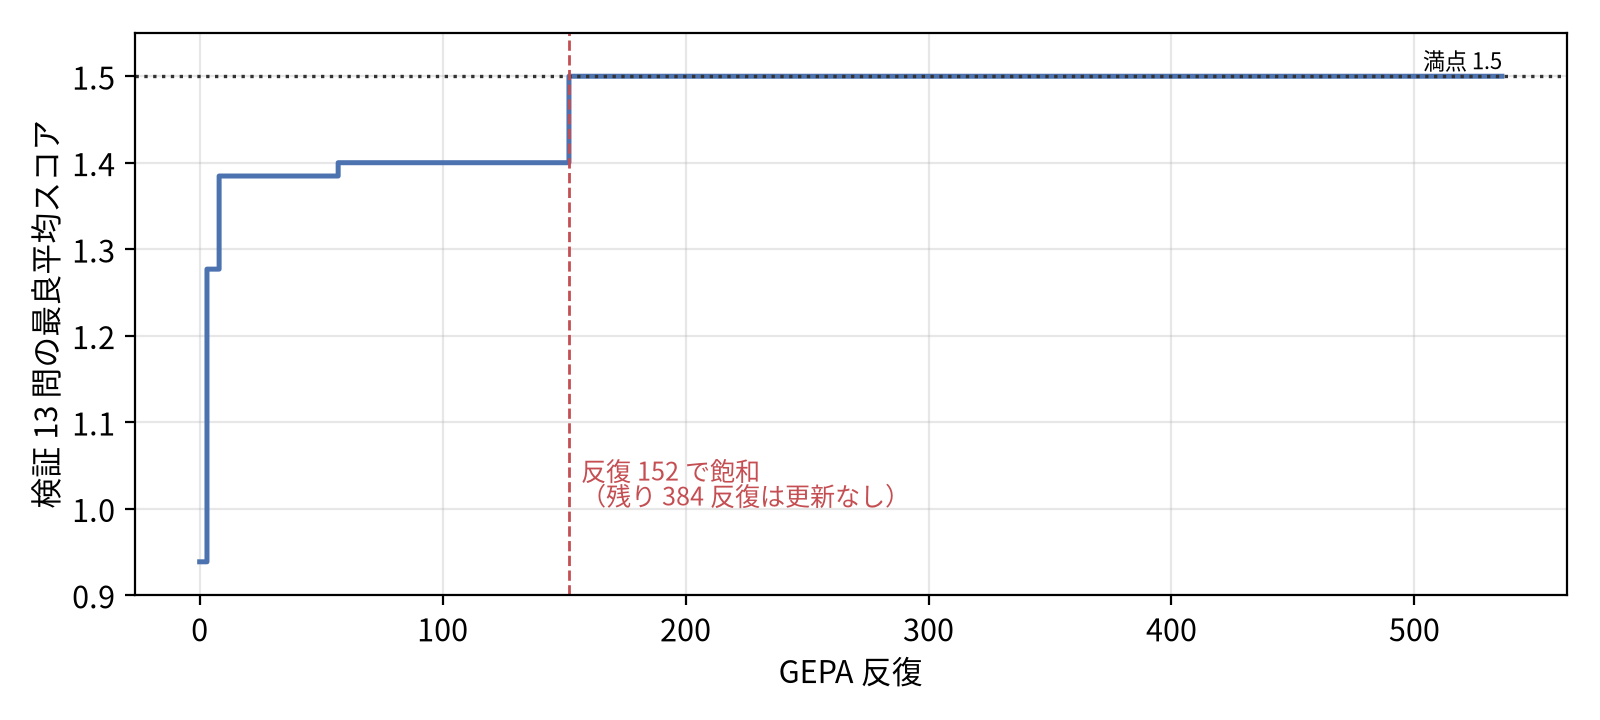
\includegraphics[width=0.95\linewidth]{./assets/gepa_val_curve.png}
  \caption{再学習GEPAの検証スコアの推移（縦軸は各時点までの最良候補の検証13問平均．破線は最良が最後に更新された反復152）}
  \label{fig:gepa}
\end{figure}


\subsection{上限の確認: Claude Fable 5.1}

同じ140問を，プロジェクトの文脈を持たないClaude Fable 5.1に問題文だけ渡すと，138問が正解で平均1.494だった（外した2問も目的値は参照と一致）．
Qwen3.6の最良条件との差は$+0.07\,[+0.01, +0.14]$しかない．
つまり，この問題集でプロンプト最適化が埋められる余地はQwen3.6で0.07前後，Qwen3.8で0.2前後で，後者の大半は思考予算（枠切れ）の問題である．


\subsection{蒸留の検証: 4B solverのSFT}

FableとQwenの正解コードを教師に，Agents-A1-4B（4.6B，Qwen3.5系）をこの問題集専用のsolverとしてLoRA学習した．
学習データは，教師コードを新しいinstanceで実行して正解を再確認できた（問題文，コード）対で，6,720対中6,619対が残った．
入力は参照値を含まない問題文，出力は思考文なしのコードのみである．
学習はH200 1枚で2時間6分．結果を表\ref{tab:sft}に示す．

\begin{table}[H]
  \centering
  \caption{特化4Bの結果（思考なし，出力枠6,144）}
  \label{tab:sft}
  \small
  \begin{tabular}{p{0.36\linewidth}lrrr}
    \toprule
    評価集合 & 条件 & 平均 & 正解 / 問題数 & 平均出力トークン \\
    \midrule
    SFTテスト140問（学習した28雛形の未知instance） & 素の4B & 0.723 & 64 / 140 & 1,776 \\
    同上 & SFT 4B & \textbf{1.487} & \textbf{138 / 140} & 470 \\
    生成140問（Qwen・Fableと同じ集合） & SFT 4B & 1.504 & 140 / 140 & 472 \\
    雛形外70問（学習に種別ごと現れない） & 素の4B & 0.602 & 27 / 70 & 2,428 \\
    同上 & SFT 4B & 0.430 & 18 / 70 & 717 \\
    \bottomrule
  \end{tabular}
\end{table}

学習した種別の未知instanceでは，素の4Bから$+0.76\,[+0.63, +0.90]$改善し，Qwen3.6 compactを有意に上回ってFableと同等になった．
140問の所要は5分である（Qwen3.6は1時間，Qwen3.8は3〜4時間）．
一方，学習にない種別の70問では$-0.17\,[-0.43, +0.09]$と向きが負だった．
学習データの表層パターン（辺の読み方，例外時に固定値を返すfallback）を別種別に当てはめる失敗が増えたためである．
特化SFTで得られるのは「学習した28種別を解く能力」であり，対象を広げるには雛形を足して再学習する必要がある．

なお，Qwen3系のchat templateは学習データに空の思考ブロックを描画するため，既定設定で推論すると思考を始めて枠を使い切る（平均0.558）．
\texttt{enable\_thinking: false}で学習時と同じ描画にして初めて1.487になる．


\subsection{蒸留元・土台モデルの選定}

より大きい土台の候補としてGemma 4 12BとMinistral 3 14B Reasoningを，4Bと同じ入力形式でzero-shot評価した（表\ref{tab:candidates}）．
Gemma 4は思考なしでQwen3.8の各条件（1.22〜1.31）と同程度に解けるが，思考ありでは139問が枠切れになる．
Ministralは思考が収束するものの，1問平均15kトークンを使って正解が23問少ない．
生成140問での差は$+0.20\,[+0.10, +0.31]$で有意であり，SFTの土台はGemma 4 12B（思考なし）にする．

\begin{table}[H]
  \centering
  \caption{候補モデルのzero-shot結果（思考なしは出力枠6,144，思考ありは65,536．雛形外72問は表\ref{tab:sft}の70問に参照解に欠陥のある2問を加えたもの）}
  \label{tab:candidates}
  \small
  \begin{tabular}{lrrrrr}
    \toprule
    モデル & 生成140問 平均 & 正解 & 枠切れ & 雛形外72問 平均 & 正解 \\
    \midrule
    Gemma 4 12B（思考なし） & \textbf{1.329} & 124 & 0 & 1.078 & 47 \\
    Gemma 4 12B（思考あり） & $-0.486$ & 1 & 139 & $-0.500$ & 0 \\
    Ministral 3 14B Reasoning & 1.126 & 101 & 11 & 1.024 & 41 \\
    \bottomrule
  \end{tabular}
\end{table}


\section{今週の予定}

\begin{itemize}
  \item Gemma 4 12Bを土台に，同じ検証済みデータでSFTし，4Bと同じ3つの評価集合で比べる
  \item 雛形を追加して学習データの種別を広げ，雛形外への汎化が伸びるか確かめる
  \item GEPAは雛形を学習用と評価用に分けて回し，見ていない種別への効果を直接測る．反省プロンプトを一般原則優先に差し替えた条件も並べる
  \item 再学習GEPAを出力枠32kで評価し，利得が「早く答えさせる」効果だけかを切り分ける
\end{itemize}


% \clearpage

\begin{thebibliography}{99}

\end{thebibliography}

% \clearpage
% % \includepdf[pages=-]{./assets/DSPy_論文解説.pdf}
% \includepdf[pages=-,fitpaper=true,pagecommand={}]{./assets/DSPy_論文解説.pdf}



\end{document}
